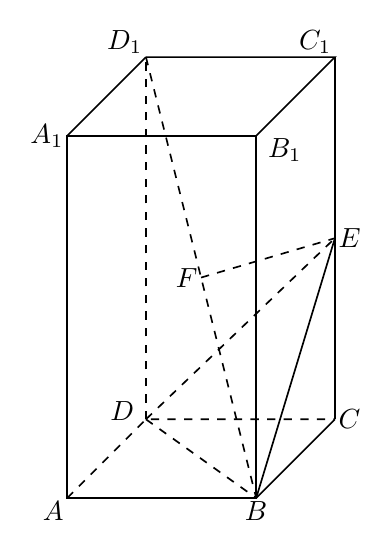
\begin{tikzpicture}[x=1cm,y=1cm,line width=.6pt,font=\normalsize]
% Upright cuboid ABCD-A1B1C1D1, E mid CC1, F mid BD1
\coordinate (A) at (0,0);
\coordinate (B) at (2.4,0);
\coordinate (C) at (3.4,1.0);
\coordinate (D) at (1.0,1.0);
\coordinate (A1) at (0,4.6);
\coordinate (B1) at (2.4,4.6);
\coordinate (C1) at (3.4,5.6);
\coordinate (D1) at (1.0,5.6);
\coordinate (E) at (3.4000000000,3.3000000000);
\coordinate (F) at (1.7000000000,2.8000000000);
% solid: front face, top, right edges, B-C, B-E
\draw (A) -- (B) -- (B1) -- (A1) -- cycle;

\draw (D1) -- (C1) -- (B1);
\draw (D1) -- (A1);
\draw (C1) -- (E) -- (C);
\draw (C) -- (B);
\draw (B) -- (E);
% hidden dashed: bottom back, A-D, D-D1, D-B, D-E, D1-B, E-F
\draw[dashed] (A) -- (D) -- (C);
\draw[dashed] (D) -- (D1);
\draw[dashed] (D) -- (B);
\draw[dashed] (D) -- (E);
\draw[dashed] (D1) -- (B);
\draw[dashed] (F) -- (E);
% labels with clearance
\node[anchor=north east,inner sep=1pt] at ([xshift=0pt,yshift=0pt]A) {$A$};
\node[anchor=north,inner sep=1pt] at ([xshift=0pt,yshift=0pt]B) {$B$};
\node[anchor=west,inner sep=1pt] at ([xshift=0pt,yshift=0pt]C) {$C$};
\node[anchor=east,inner sep=1pt,xshift=-3pt,yshift=3pt] at ([xshift=0pt,yshift=0pt]D) {$D$};
\node[anchor=east,inner sep=1pt] at ([xshift=0pt,yshift=0pt]A1) {$A_{1}$};
\node[anchor=west,inner sep=1pt,xshift=3pt,yshift=-5pt] at ([xshift=0pt,yshift=0pt]B1) {$B_{1}$};
\node[anchor=south east,inner sep=1pt] at ([xshift=0pt,yshift=0pt]C1) {$C_{1}$};
\node[anchor=south east,inner sep=1pt] at ([xshift=0pt,yshift=0pt]D1) {$D_{1}$};
\node[anchor=west,inner sep=1pt] at ([xshift=0pt,yshift=0pt]E) {$E$};
\node[anchor=east,inner sep=1pt] at ([xshift=0pt,yshift=0pt]F) {$F$};
\end{tikzpicture}
